\documentclass{llncs}

\usepackage{url}
\usepackage{graphicx}
\usepackage{listings}
\usepackage{verbatim}
\usepackage[lined,linesnumbered,algochapter]{algorithm2e}
\usepackage{tikz}
\usetikzlibrary{arrows,automata}
\usepackage{xspace}
\usepackage{todonotes}          % Package for working draft comments
\usepackage{hyperref}           % Package for hyperlink references in the document

\usepackage[english]{babel}

\setcounter{secnumdepth}{2}
\setcounter{tocdepth}{3}

% define custom macros for specific formats or names
\newcommand{\uml}[1]{\texttt{#1}}
\newcommand{\cd}{\textsf{Class Diagram}}

%Colors for general listings
\definecolor{mygreen}{rgb}{0,0.6,0}
\definecolor{mygray}{rgb}{0.5,0.5,0.5}
\definecolor{mymauve}{rgb}{0.58,0,0.82}
%Colors for JSON listings
\colorlet{punct}{red!60!black}
\definecolor{background}{HTML}{EEEEEE}
\definecolor{delim}{RGB}{20,105,176}
\colorlet{numb}{magenta!60!black}

\lstset{ %
   backgroundcolor=\color{background},   % choose the background color; you must add \usepackage{color} or \usepackage{xcolor}
   basicstyle=\small\ttfamily,        % the size of the fonts that are used for the code
%   breakatwhitespace=false,         % sets if automatic breaks should only happen at whitespace
%   breaklines=true,                 % sets automatic line breaking
  captionpos=b,                    % sets the caption-position to bottom
  commentstyle=\color{mygreen},    % comment style
%   deletekeywords={...},            % if you want to delete keywords from the given language
%   escapeinside={\%*}{*)},          % if you want to add LaTeX within your code
%   extendedchars=true,              % lets you use non-ASCII characters; for 8-bits encodings only, does not work with UTF-8
   frame=lines,                    % adds a frame around the code
%   keepspaces=true,                 % keeps spaces in text, useful for keeping indentation of code (possibly needs columns=flexible)
  columns=fixed,
  keywordstyle=\color{mymauve},       % keyword style
  stringstyle=\color{blue},
%   morekeywords={*,...},            % if you want to add more keywords to the set
  numbers=left,                    % where to put the line-numbers; possible values are (none, left, right)
  numbersep=5pt,                   % how far the line-numbers are from the code
  numberstyle=\scriptsize\color{mygray}, % the style that is used for the line-numbers
%   rulecolor=\color{black},         % if not set, the frame-color may be changed on line-breaks within not-black text (e.g. comments (green here))
 showspaces=false,                % show spaces everywhere adding particular underscores; it overrides 'showstringspaces'
 showstringspaces=false,          % underline spaces within strings only
 showtabs=false,                  % show tabs within strings adding particular underscores
%   stepnumber=2,                    % the step between two line-numbers. If it is 1, each line will be numbered
  tabsize=2,                       % sets default tabsize to 2 spaces
%   title=\lstname                   % show the filename of files included with \lstinputlisting; also try caption instead of title
}


\begin{document}
\renewcommand{\thelstlisting}{\arabic{lstlisting}}
\pagestyle{plain}
\pagenumbering{roman}

\title{Refactoring UML models: Co-refactoring class diagrams and activity diagrams conform to fUML}


\author{Sebastian Geiger (1127054) \and Kristof Meixner (9725208)}
\institute{Business Informatics Group\\Vienna Technical University}
\maketitle

\begin{abstract}
In this work we will present ideas and concepts for the refactoring of fUML models. The main contribution of this work is 
the extension of existing UML refactorings to cover not only the static aspect of UML such as class diagrams but to also 
include refactorings for dynamic
parts such as activity diagrams. In this work we will present basic concepts for refactoring of models with EMF and show how model semantics can be
preserved through the use of OCL constraints. In the remainder of the paper we then present our toolchain and the used technologies
of EMF (in particular Ecore and OCL) and how we used them for refactoring of models. We also present a discussion of EMF Refactor, which shows how such refactorings
can be made available in the Eclipse GUIs such as the UML tree editor or Papyrus.
\end{abstract}

\tableofcontents
\newpage

\pagenumbering{arabic}

\section{Introduction}
% INTRODUCTION Models are getting more important in model-based software development, model-driven software development,
% model-driven architecture Models thus need to have a good quality

Model-based software development or model-driven software development is not only an extensive field of research but
also receives increased attention from the industry. Nowadays models are not only used as visual explanations of
software concepts but as source for the development process itself. Thus models need to provide an abstraction of
the represented domains in a high quality. Mohagheghi \textit{et al.} \cite{DBLP:journals/infsof/MohagheghiDN09} discussed 
quality attributes like \textit{Correctness}, \textit{Completeness} and \textit{Consistency} of models in their work.

% UML is a modelling language for models provided by the OMG that supports various types of models

To represent models in a more formal way the \textit{Object Management Group} (OMG) developed the \textit{Unified Modeling Language} (UML) 
\cite{man:UML} which by now advanced to an industry standard for 
modeling. UML provides an abstract syntax of the modeling concepts and rules how to combine them, an explanation 
of the semantics of the concepts as well as a specification of the notation elements in human-readable form.
Build on these common concepts models can be preserved over time and even be reused due to their formalized semantics. Nevertheless models 
might have to be revised over the lifecycle of the software. With todays trend to more agile software 
development such as eXtreme Programming \cite{DBLP:journals/computer/Beck99} or Scrum \cite{DBLP:journals/software/RisingJ00} 
changes on models have to be even more efficient which brings refactoring of models into the focus of research.

% Refactoring is behavior preserving changing that should also improve quality

Refactoring is a technique that originates from source code development but can also be applied to model engineering.
The goal is to introduce behavior preserving changes \cite{mast:REFOOF} that increase the quality and understandability
of the models.

% Refactoring must preserve the behavior of all model types

While refactoring source code and textual code respectively applies to a single type of representation, in UML different
types of diagrams exist to represent various aspects of the models. This makes behavior preserving refactoring even harder 
as it needs to span over those different types of diagrams and semantics.

% Behaviour preservation can be tested statically or dynamically UML can be analysed statically fUML is a modelling
% language for models provided by the OMG that also allows execution and thus can be analysed dynamically

Different approaches exist to prove the semantic preservation of refactorings. One is the static analysis of
UML models via metrics which can be done with
the \textit{Object Constraint Language} (OCL) \cite{man:OCL}. Another way is to verify that models can be executed and to compare 
different attributes of the execution like input and output values, execution traces or states of the 
original and refactored models. The OMG introduced a foundational subset 
of UML metamodel concepts abbreviated fUML \cite{man:FUML} and precisely defined the semantics for their execution. Thanks 
to this standard compliant UML models can be transformed to an executable form. 
Furthermore in \cite{DBLP:conf/icse/Mayerhofer12} Mayerhofer \textit{et al.} proposed a framework based on fUML that is able to execute
and debug models that conform to fUML.

% our approach is to combine both

The goal of this work is to introduce refactorings for fUML models, examine the requirements for co-refactoring of the
corresponding diagram types and define which co-changes have to be performed to preserve the behavior. Our approach to
verify
the semantic preservation of the models is twofold. On the one hand we use OCL pre- and postconditions
\cite{rob99} to determine whether a refacoring can be applied and whether the models are semantically correct afterwards.
On the other hand the models have to stay executable after the changes.

% we present a motivating example (class and activity diagrams) we provide some refactorings that target bothe diagram
% types we provide a how to test statically and dynamically, then refator and retest we provide a toolchain

% we provide some related work we provide a conclusion

The rest of the work is structured as follows. Section \ref{sec:motivation} gives an introduction to fUML and shows how 
the preservation of semantics can be achieved during refacoring. 
Section \ref{refactoring-examples} describes a selection of useful refactorings inspired by Fowler \cite{fow99} and 
Markovic and Baar \cite{DBLP:journals/sosym/MarkovicB08} and their effects on class diagrams as
well as activity diagrams. We also provide a motivating example of a model that is used throughout the paper. In Section 
\ref{sec:fuml-refactoring} we show which pre- and postcondition are needed for the refactorings and
how we refactor the models. In Section \ref{sec:toolchain} we describe the toolchain that we use to define the models, 
implement a set of refactorings and test them. Section \ref{sec:limitations} describes which limitations our work has. 
Related work is covered in Section \ref{sec:relatedwork} and a conclusion is drawn in 
Section \ref{sec:conclusion} to summarize the paper.

% what is refactoring and what does it mean in the context of models?
% what is fuml? what does fuml consist for diagram types?
% what is ocl? why do we use it and what for?

%fUML adds semantics to UML models that make it possible to create semantically closed models which can be executed on the model level. With
%fUML classic refactorings are not enough to refactor those models as they do not support the refactoring of the dynamic aspects of models
%such as activity diagrams.

\section{Motivation}
\label{sec:motivation}
% what do we want to achieve?
fUML is a subset of UML for which additional semantics are defined such that models can be executed. The subset contains concepts
of the packages \textit{Classes}, 
\textit{CommonBehaviors}, \textit{Activities} and \textit{Actions}, which basically means someone can create 
\textit{class diagrams} and \textit{activity diagrams} with fUML.

If a refactoring 
is performed on a UML model such as a class diagram, then any activity diagram which is releated to the class diagram, has 
to be checked and possibly changed as well. In Section \ref{sec:fuml-refactoring} we will present some examples of fUML 
activity diagrams and present the implications that result from changing class 
diagrams (a procedure called \textit{co-refactoring}).

Since a refactoring changes the structure of a model it is important to ensure that all changes maintain the original 
semantics of the model. Violating this requirement can result in models with either a different behavior, or in models 
which can no longer be executed. To ensure semantic preservation, two main techniques can be used. First, the refactoring 
can be broken down into smaller steps, each of which either guarantees to preserve the semantics of the model or makes it 
easier to verify that this is the case. Second, logical constraints can be used to limit refactorings on models to only 
those cases where semantic preservation can be ensured. For this purpose pre- and postconditions are specified with OCL 
constraints. A refactoring is then only applied if the original model satisfies the precondition before the refactoring is 
applied and the postcondition after the refactoring has been completed. Such constraints must be individually specified 
for each kind of refactoring that is to be performed. In this paper we introduce and discuss different OCL constraints 
for the refactorings that we introduce.

Refactorings are only useful if they can be easily applied to the models through an easy to use process such as a 
graphical front end. EMF Refactor\footnote{\url{http://www.eclipse.org/emf-refactor/}} allows the integration of 
refactorings into editors such as the UML tree editor or 
Papyrus\footnote{\url{http://www.eclipse.org/papyrus/}}. EMF Refactor provides a Java API as well as a module 
concept to integrate refactorings. We will discuss the use 
of EMF Refactor as part of our tool chain presentation.

%TODO: Maybe discuss emf.refactor as part of future work?

% Why is it interesting to refactor models
% Why is it important in fUML that models remain consistent -> to preserve executability
% It is possible to use pre and post conditions in OCL to guarantee the semantic preservation of models during refactorings.

\section{Refactoring examples}
\label{refactoring-examples}
% take model refactorings of markovic paper
% insurance example
% create example that supports all proposed refactorings

This section covers some refactorings of fUML models as well as a fUML model which we use as an example for this work. 
Markovic \cite{DBLP:journals/sosym/MarkovicB08} presented a list of refactorings for class 
diagrams and co-refactoring of OCL constraints. However they do not consider other diagram types and possible co-refactorings between 
them. Nevertheless we use this catalog as an input and adapt it for our use case. The resulting list of 
refactorings which we plan to evaluate and implement is shown in Figure \ref{fig:refactoringlist}. The first column shows 
whether a change in the abstract syntax tree is necessary for this refactoring. No means that the change does not directly 
affect the structure of the abstract syntax, for example because it does not change cross references between objects or 
only modifies properties of the objects. A refactoring of a class 
diagram can make corresponding changes in the associated activity diagrams necessary. These so called co-refactorings are 
necessary if the abstract syntax tree changes in such a way, that references in activity diagrams become invalid. This is 
for example the case if properties or operations are removed or become private. A more detailed explanation of
co-refactorings is given in Section \ref{sec:fuml-refactoring} together with the introduction of each refactoring.

\begin{figure}[h!t]
 \centering
 \begin{tabular}[]{l | c | c}
  Class diagram refacoring & Abstract syntax changes & Activity diagram co-refacoring\\
  \hline
  Encapsulate property & Yes & Yes\\
  Extract class & Yes & Yes\\
  Extract superclass & Yes & No\\
  Pull up association end & Yes & Yes\\
  Pull up property & Yes & Yes\\
  Pull up operation & Yes & Yes\\
  Remove unused class & No & No\\
  Rename class & No & No\\
  Rename operation & No & No\\
  Rename property & No & No\\
 \end{tabular}
 \caption{Considered refactorings}
 \label{fig:refactoringlist}
\end{figure}

\begin{figure}[h!t]
 \centering
 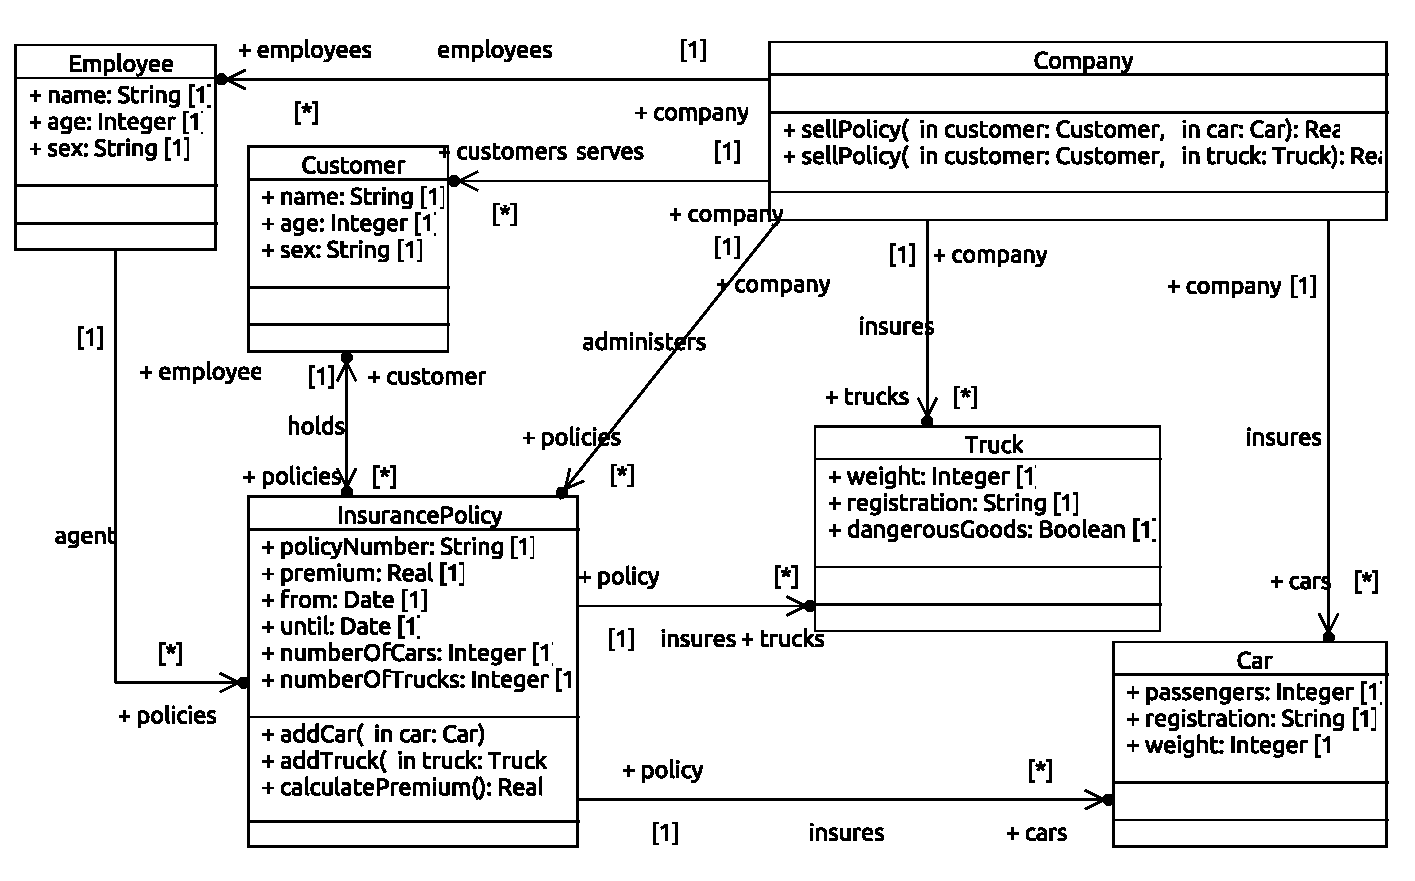
\includegraphics[scale=0.5]{images/insurance/Model_Model_ClassDiagram.PDF}
 \caption{Insurance class diagram before refactoring}
 \label{fig:classdiagramcomplex}
\end{figure}

In order to demonstrate how the presented refactorings affect both class and activity diagrams we will present an example 
model from the insurance domain. In the insurance business there are domain objects such as an insurance policy. Cars and 
trucks can be insured by adding them to the policy. There is an insurance company which has customers and employees where customers may purchase an insurance policy 
for their cars or trucks. Figure \ref{fig:classdiagramcomplex} shows a class diagram of such an insurance company. This class 
diagram would benefit from several possible refactorings such as an \textit{extract superclass} which can be applied to both \texttt{Car} 
and \texttt{Truck} to extract a \texttt{Vehicle} class. A simple \textit{extract class} can be used on \texttt{InsurancePolicy} to 
extract the \texttt{from} and \texttt{until} dates into an own \texttt{InsurancePeriod} class. As part of the 
\textit{extract superclass} refactoring two additional refactorings namely \textit{pull up property} and \textit{pull up operation} are 
used to move the identical properties and operations of both classes to the new superclass. As the 
properties \texttt{weight} and \texttt{registration} are public, we can use \textit{encapsulate field} to make them private and 
provide getter and setter implementations. Finally the operation \texttt{addCar} can be renamed into \texttt{addVehicle} with \textit{rename operation} 
and the \texttt{addTruck} operation can be removed with \textit{remove operation}\footnote{\textit{remove operation is not covered by our paper}}. Finally Figure \ref{fig:classdiagramcomplexRef} shows 
the refactored class diagram.

\begin{figure}[h!t]
 \centering
 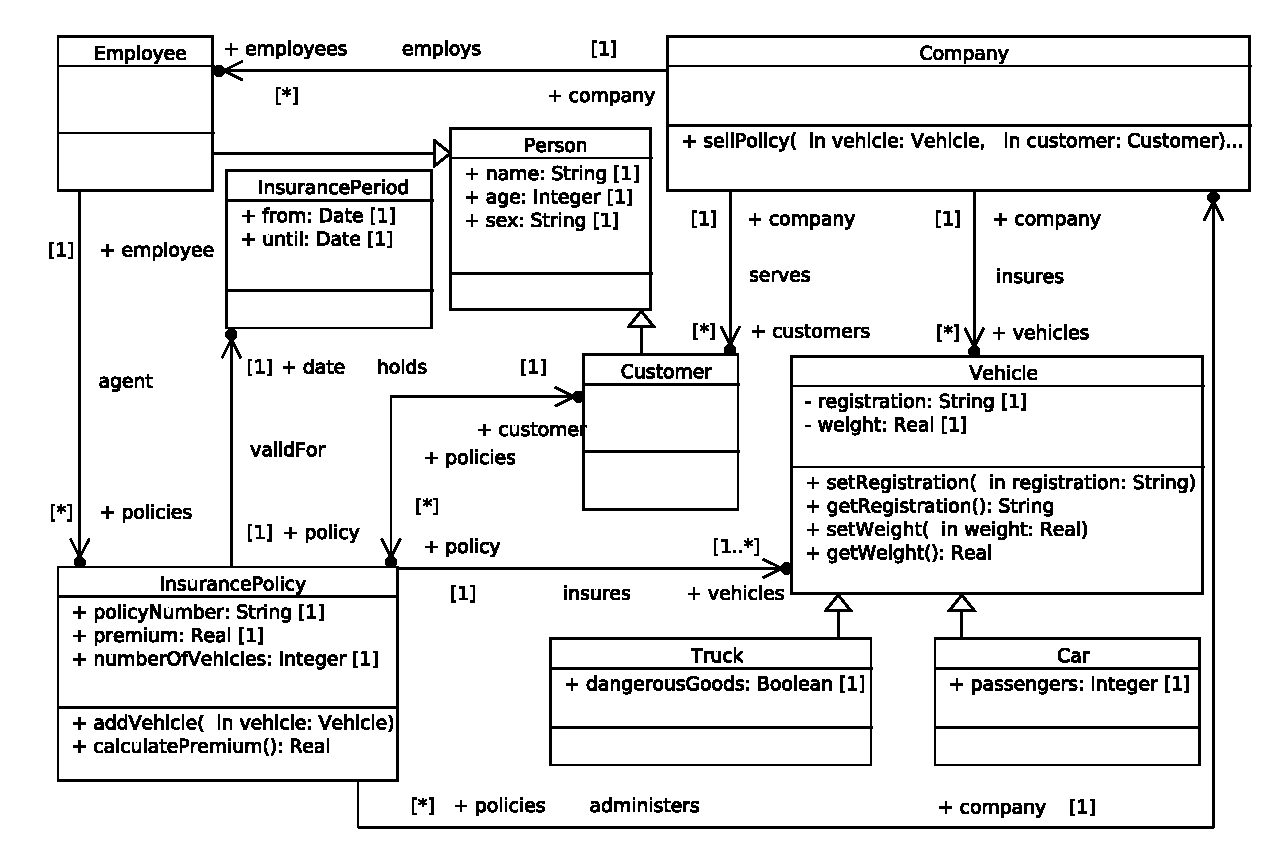
\includegraphics[scale=0.5]{images/insurance_ref/Model_Model_ClassDiagram}
 \caption{Insurance class diagram after refactoring}
 \label{fig:classdiagramcomplexRef}
\end{figure}

For each of the operations in the \texttt{InsurancePolicy} class a separate activity diagram exists which defines the behavior 
of the respective operations. As some of them are quite similar we will present only the diagrams for \texttt{addCar} in Figure 
\ref{fig:addCar} and \texttt{calculatePremium} in  Figure \ref{fig:calculatePremium}.

The activity for the \texttt{addCar} operation works as follows. It reads the policy with a \texttt{Read\-Self\-Action}, takes the 
car as a parameter and uses the \texttt{Add\-Structural\-Feature\-Value\-Action} to add the car to the insurance policy. In parallel 
it reads the number of cars in the policy with \texttt{Read\-Structural\-Feature\-Value\-Action}, specifies an integer
with a value of '1' with 
a \texttt{Value\-Specification\-Action}, adds the numbers with a \texttt{Call\-Behavior\-Action} and writes it back to the 
\texttt{numberOfCars} variable with another \texttt{Add\-Structural\-Feature\-Value\-Action} that replaces the old value.

The \texttt{calculatePremium} activity is more complex, it calculates the insurance premium as described below:

\begin{itemize}
 \item Read the policy with a \texttt{Read\-Self\-Action}.
 \item Read the number of cars and trucks with \texttt{Read\-Structural\-Feature\-Value\-Action}.
 \item Add the two numbers up with a \texttt{Call\-Behavior\-Action}, which invokes the opaque behavior 'add'.
 \item Multiply the result in a \texttt{Call\-Behavior\-Action} with a base premium value specified in a \texttt{Value\-Specification\-Action}.
 \item Read the age of customer of the policy with two actions of type \texttt{Read\-Structural\-Feature\-Value\-Action} in a row.
 \item Decide whether the age of a customer is below a certain age and define a base value or supplement with a \texttt{Value\-Specification\-Action}.
 \item Multiply the value and the result of the calculation above and return it.
\end{itemize}

\begin{figure}[h!t]
 \centering
\makebox[\textwidth]{
 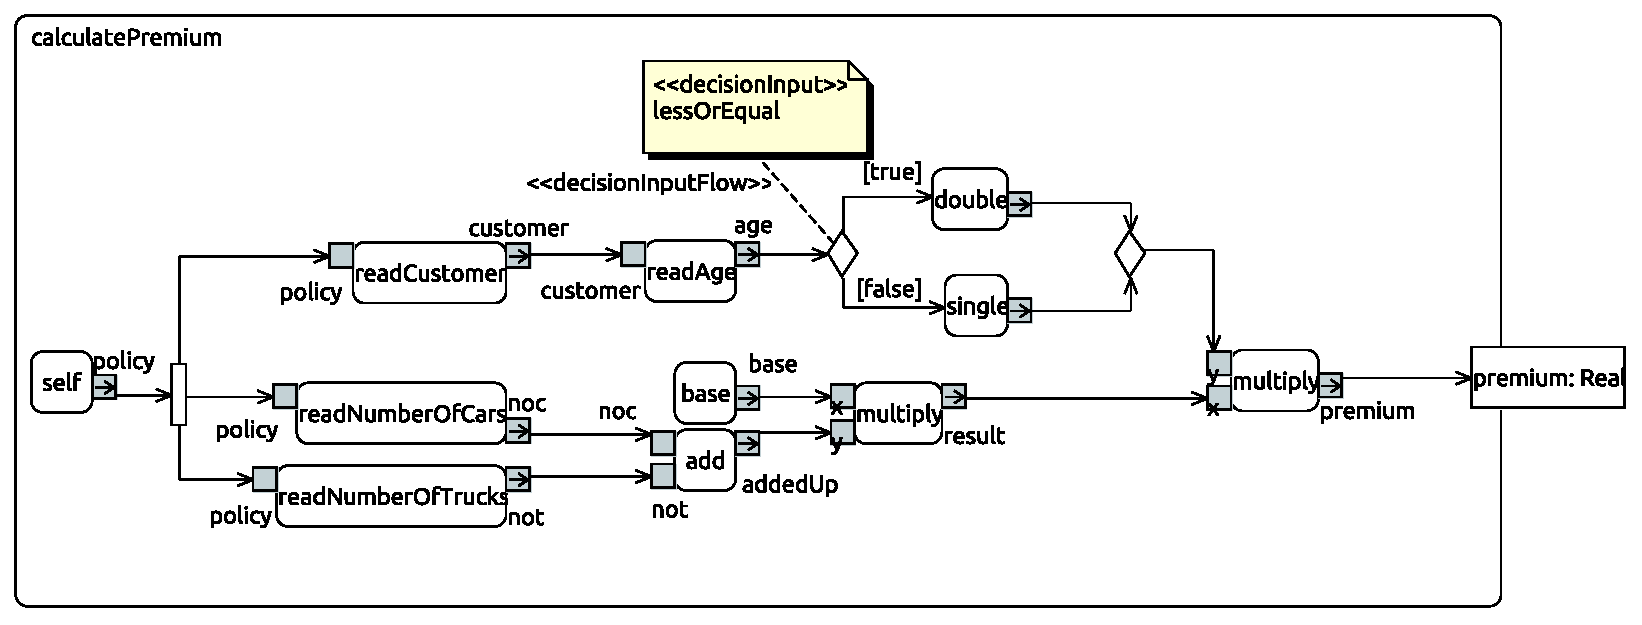
\includegraphics[scale=0.5]{images/insurance/Activity_calculatePremium_calculatePremium}
}
 \caption{Activity diagram of the operation \texttt{calculatePremium} before co-refacoring}
 \label{fig:calculatePremium}
\end{figure}

\begin{figure}[ht]
 \centering
\makebox[\textwidth]{
 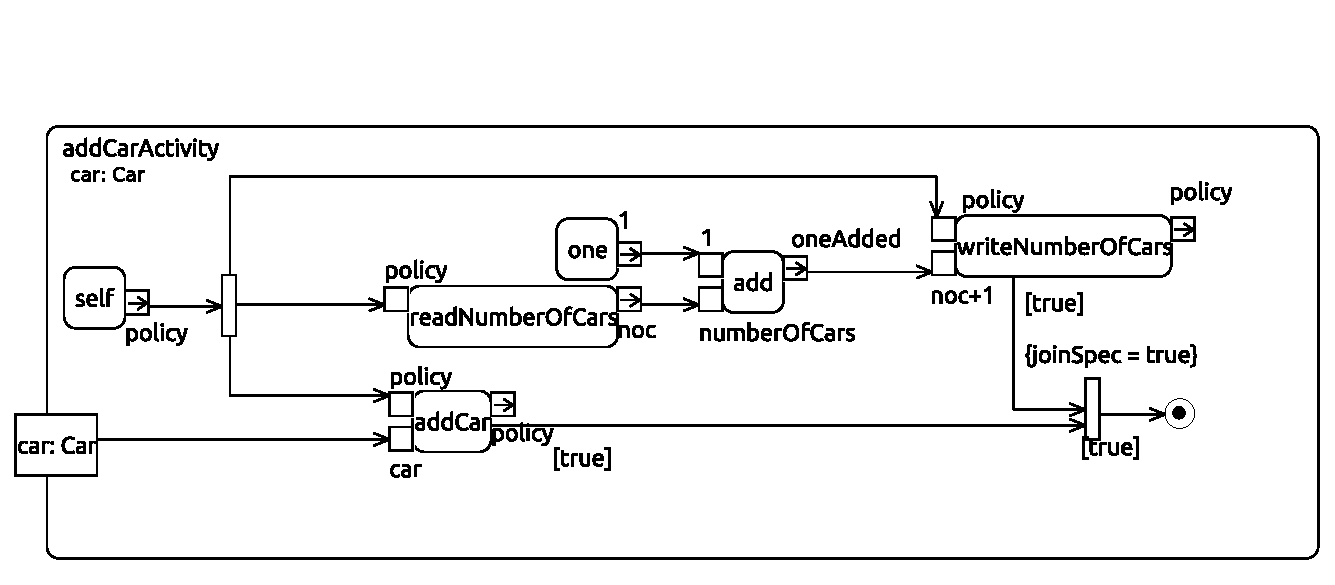
\includegraphics[scale=0.6]{images/insurance/Activity_addCarActivity_addCarActivity}
}
 \caption{Activity diagram of operation \texttt{addCar} before refactoring}
 \label{fig:addCar}
\end{figure}

Figure \ref{fig:calculatePremiumRef} shows how the activity diagram of the operation \texttt{calculatePremium} benefits from a refactoring of the corresponding 
class diagram. Additionally a new activity diagram for the \texttt{addVehicle} operation instead of the old 
\texttt{addCar} and \texttt{addTruck} diagrams was created shown in Figure \ref{fig:addCarRef}. It is rather obvious 
that the complexity of both diagrams decreased on the visual level.

\begin{figure}[h!t]
 \centering
 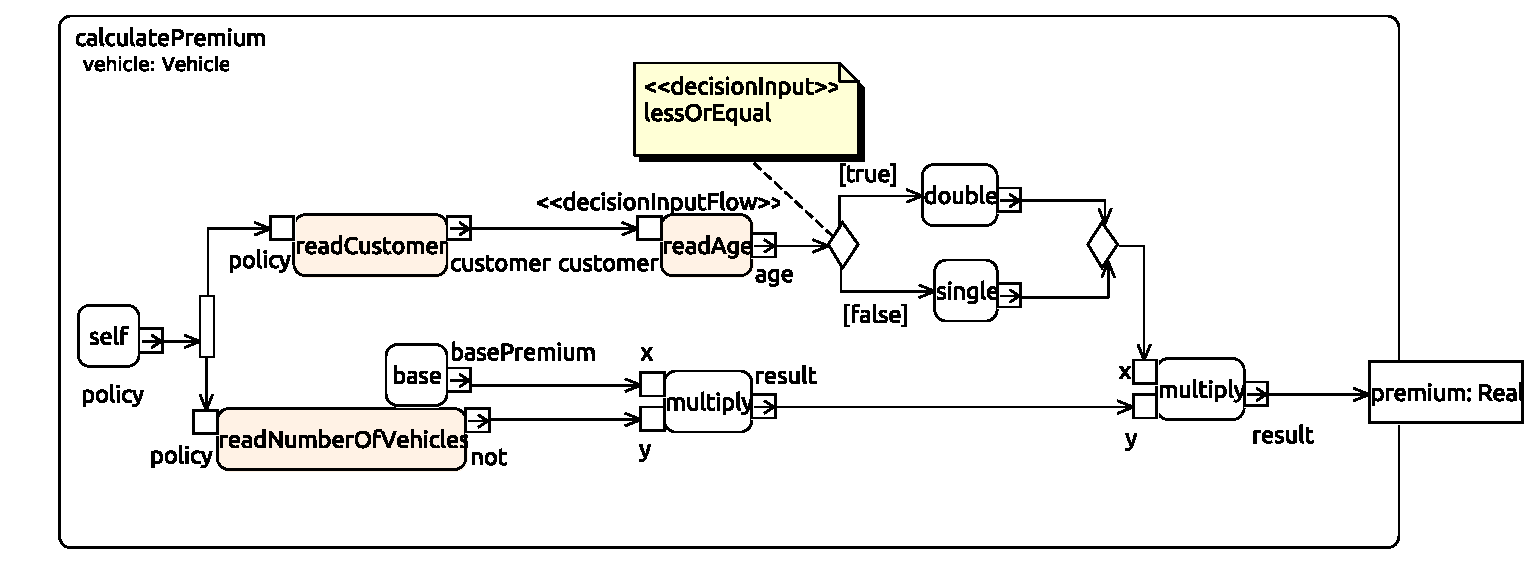
\includegraphics[scale=0.5]{images/insurance_ref/Activity_calculatePremium_calculatePremium}
 \caption{Activity diagram of the operation \texttt{calculatePremium} after co-refactoring}
 \label{fig:calculatePremiumRef}
\end{figure}

\begin{figure}[h!t]
 \centering
 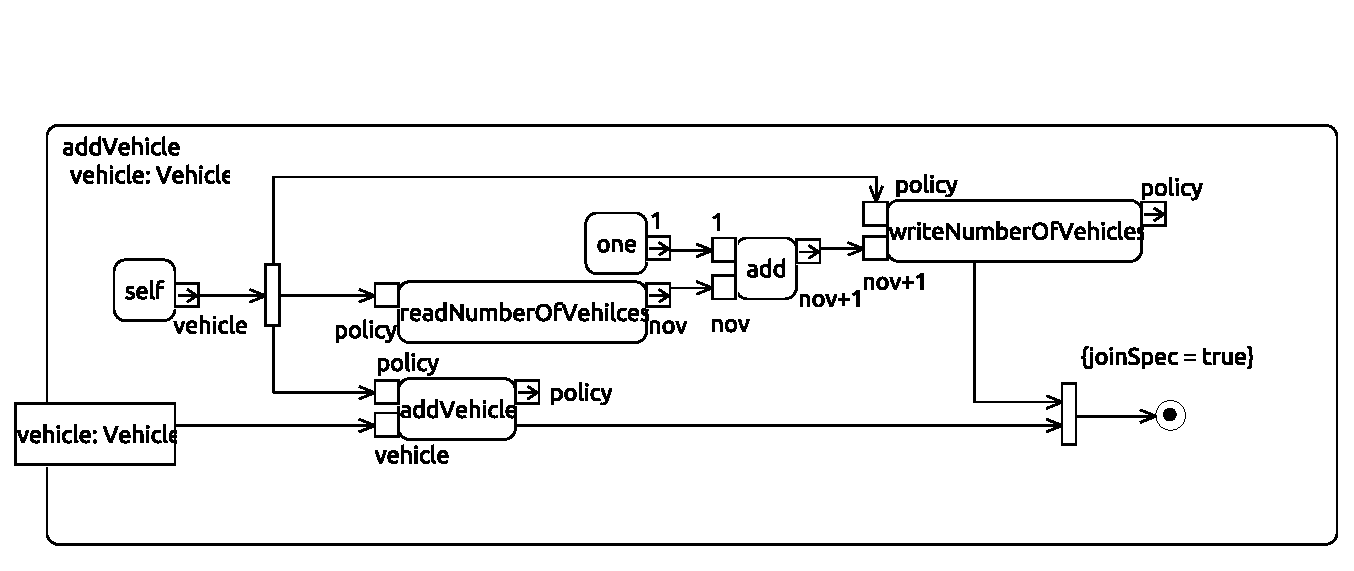
\includegraphics[scale=0.6]{images/insurance_ref/Activity_addVehicle_addVehicle}
 \caption{Activity diagram of operation \texttt{addVehicle} resulting from the refactoring}
 \label{fig:addCarRef}
\end{figure}

\section{Refactoring of fUML models}
\label{sec:fuml-refactoring}
% abstract syntax of fUML and changes in diagrams
% ecore and ocl (with code examples

In the last section we presented an example fUML model comprising a class diagrams and several activity diagrams. We also presented some of the possible 
refactorings such as \textit{extract superclass} on the class diagram and their impact on the activity diagrams. In this 
section we discuss how the syntax of the models actually need to be transformed in order to realize the refactoring. Furthermore we describe 
the refacorings from the prior section in detail.

Every model has two kinds of syntaxes. The concrete syntax (or notation), which defines how the model is visualized, and the abstract
syntax, which defines the UML language elements and the grammar of the model. In order to refactor a model, we need to look 
at its abstract syntax and transform it according to the refactoring rules.

\subsection{Rename class, rename property \& rename operation}
\label{sec:renames}
A refactoring takes several parameters to configure the parts of the model that change. Rename 
refacorings need the model element that shall be refactored as well as the new name as parameter. The respective classes, operations and properties can then be adapted 
and the direct references be changed as the abstract syntax representation does not change. However in order to guarantee that the 
refactoring is possible, we have to ensure that there are no occurrences of the same type with the same name as the 
new name. In this work we did not take techniques such as operation overloading into account. In our example there is 
no such case explicitly included.

\begin{lstlisting}[language=OCL,caption=OCL for rename property,label=lst:renameproperty]
context Property:
pre:  self.class.attribute->union(
          self.class.allParents().attribute)
      ->forAll(a|a.name <> 'newAttributeName')
\end{lstlisting}

\begin{lstlisting}[language=OCL,caption=OCL for rename operation,label=lst:renameoperation]
context Operation:
pre:  self.class.ownedOperation
      ->union(self.class.allParents()
              ->selectByType(Class).ownedOperation)
      .isDistinguishableFrom(newOperation, self.namespace)
\end{lstlisting}

\begin{lstlisting}[language=OCL,caption=OCL for rename class,label=lst:renameclass]
context Class:
pre:  self.namespace.member
      ->selectByType(Class)
      ->forAll(c | c.name <> 'newClassName')
\end{lstlisting}

The post conditions for rename property apply to all \texttt{Structural\-Feature\-Action} objects
which reference the renamed property. For rename operation it applies to all \texttt{Call\-Operation\-Action} objects which
call the renamed operation. For rename class all elements which reference objects of the renamed class must reference
the new class name, that includes objects such as \texttt{Parameter} or \texttt{Pins} (InputPin, OutputPin).

\subsection{Extract superclass}
\label{sec:extract}
The \textit{extract superclass} refactoring takes two parameters, the new name of the extracted superclass as well as
the list of classes that participate in the refactoring and which will receive the new class as their superclass.

In terms of the abstract syntax of these models, the two classes \texttt{Car} and \texttt{Truck} are instances of 
type \textit{Class} of the meta-model a superclass named \texttt{Vehicle} would be an instance of type \textit{Class} as well, 
and can be associated with these two classes through the recursive attribute \textit{general} of the class \textit{Class} 
to create the inheritance hierarchy. However the abstract syntax representation of the diagram does not change. In order to 
achieve a correct refactoring each class that participates in the refactoring must not already have a superclass. The 
model would also benefit from changing all possible references to the new class.

\begin{lstlisting}[language=OCL,caption=OCL for extractSuperclass refactoring,label=lst:extractsuperclass]
context Class:
pre:  self.namespace.member
      ->selectByType(Class).name
      ->forAll(o | o <> 'nameOfClassToExtract')
post: newSuperClass.visibility = uml::VisibilityKind::public
      and self.general->includes(newSuperClass)
\end{lstlisting}

% Fehlende Constraints hinzufuegen
% Zusaetzliche interessante refactorings
% Execution of models (theoretisch, evtl. praktisch)
% Co-refactoring only from class to activity diagrams, not vice versa.
% Refactoring looses concrete syntax representation (e.g. model cannot be opened with papyrus).

\subsection{Pull up property \& pull up operation}
\label{sec:pullup}
Both refactorings are quite similar which is why we describe the first and explain the specifics for the latter one afterwards. 
There are two cases of the \textit{pull up property} refactoring. It can either be executed for a property that occurs in 
a single class or in multiple classes where the properties should also be combined and pulled up. In the class diagram 
the property has to be pulled up and the occurrences of the properties in the subclasses have to be deleted. The 
activity diagrams needs to change occurrences of the \texttt{StructuralFeatureValueAction} and use the property of 
the super class.

For the \textit{pull up operation} refactoring all \texttt{Call\-Operation\-Action} actions have to be adapted like described 
above. A precondition for both of these refactorings is that there does not already exist an property or a operation with the same name 
in the target class and that they are not private.

\subsection{Encapsulate property}
\label{sec:encapsulate}
The \textit{encapsulate property} refactoring is a rather complex one. At first setter and getter operations for the property have to be 
created. Afterwards the occurrences of the property have to be changed either to the setter for value assignments and to the getter 
for value usage. For the activity diagram the \texttt{Write\-Structural\-Feature\-Value\-Action} has to be changed to a 
\texttt{Call\-Operation\-Action} which is a \texttt{BehavioralFeature} class instead of a \texttt{StructuralFeature} class in 
the meta-model. Finally the affected property has to be set to private. The precondition for this refactoring is that there are no 
operations with the same name in the classes that use the property.

\begin{lstlisting}[language=OCL,caption=OCL for encapsulate property,label=lst:encapsulateproperty]
context Property:
pre:  self.visibility <> uml::VisibilityKind::private and
      self.class.ownedOperation
      ->forAll(o | o.isDistinguishableFrom(setOperation,
              self.namespace) and
      o.isDistinguishableFrom(getOperation, self.namespace))
\end{lstlisting}

%TODO: explain and state ocl constraints for: 
%   * Extract class
%   * Pull up association end
%   * Remove unused class

\section{Toolchain and implementation}
\label{sec:toolchain}
For our toolchain we have relied on the moliz\footnote{http://www.modelexecution.org} repository, mainly for the ability to execute the fUML 
models in a virtual machine. The models are stored in XMI format and loaded with an EMF ResourceSet. The ResourceSet
can be used to retrieve a Resource object through an URI, which is then used to access the different objects in the model 
(see Listing \ref{lst:resourceset}). All elements contained in the model are instances of Ecore (the implementation of
the MOF meta-meta-model) and they represent classes of the UML meta-model, which is implemented with Ecore.

\begin{lstlisting}[language=Java,caption=Getting the resourceset,label=lst:resourceset]
resourceSet = new ResourceSetImpl();
resourceSet.getPackageRegistry().put(UMLPackage.eNS_URI,
                                     UMLPackage.eINSTANCE);
resourceSet.getResourceFactoryRegistry()
    .getExtensionToFactoryMap()
    .put(UMLResource.FILE_EXTENSION,
         UMLResource.Factory.INSTANCE);
File file = new File(umlModelFile);
URI uri = URI.createFileURI(file.getAbsolutePath());
    resource = resourceSet.getResource(uri, true);
\end{lstlisting}

\subsection{Model refactoring}
Our refactorings are implemented with a strategy pattern, where each refactoring implements a \texttt{Refactorable}
interface that has three operations \texttt{checkPrecondition}, \texttt{performRefactoring}, and \texttt{checkPostcondition}. 
Each refactoring identifies the model objects that participate in the refactoring and then creates and evaluates the \textit{OCL} 
constraints on these objects. An object to type \texttt{OCL} from the org.eclipse.ocl package is used to create and evaluate the 
queries as can be seen in Listing \ref{lst:ocl}.

\begin{lstlisting}[language=Java,caption=OCL validation in Java,label=lst:ocl]
variable = ExpressionsFactory.eINSTANCE.createVariable();
variable.setName("newSuperClass");
variable.setType(UMLPackage.Literals.CLASSIFIER);
ocl.getEnvironment().addElement(variable.getName(),
                                variable, true);
query = helper.createQuery(
    "self.general->includes(newSuperClass)");
eval = ocl.createQuery(query);
eval.getEvaluationEnvironment()
    .add("newSuperClass", superClass);
if (!eval.check(clazz))
    return false;
\end{lstlisting}

% how to apply queries and changes?
% how to load models?
We have used \textit{OCL} notation to specify all constraints, but in the actual implementation of the refactorings it
is also possible to verify some of these constraints directly on the model by checking properties of the abstract syntax
and not use the \textit{OCL} validation facilities. One example is the constraint that verifies that the new super class does not
yet exist in the model.

If the preconditions are satisfied the actual refactoring is performed through a direct modification of the model object.
A new \texttt{Class} instance with the name of the new superclass is created and added to the model. 

%TODO: give a one line example of how a class is created?
\begin{lstlisting}[language=Java,caption=UML element creation,label=lst:createclass]
Class superClass = UMLFactory.eINSTANCE.createClass();
superClass.setName(newSuperClassName);
\end{lstlisting}


Then the existing
classes of the model are filtered to select the ones that receive the new generalization, and the newly create superclass
is added.

\subsection{Model execution}
\label{sec:execution}
% usage of fUML reference implementation of BIG
% how to execute models?
In the prior section we discussed how the models are statically examined with \textit{OCL} constraints if a refacoring 
is applicable. In this section we will show how the models can be tested dynamically by executing them. We use the 
reference implementation as described in \cite{DBLP:conf/models/MayerhoferLK12} to execute the activity diagrams of 
our models.

\begin{lstlisting}[language=Java,caption=Converting the UML diagram to fUML,label=lst:conversion]
NamedElement namedElement = obtainFirstNamedElement();
IConverter converter = getConverter(namedElement);
IConversionResult conversionResult = converter
  .convert(namedElement);
Activity activity = conversionResult.getActivity(name);
\end{lstlisting}

Our models are formally created in \textit{UML} and are converted to \textit{fUML} with the \texttt{UML2fUML} converter 
provided by the implementation as shown in Listing \ref{lst:conversion}. The resulting \textit{fUML} diagram is executed in the 
virtual machine for model execution. 
We test our models by examining if a complete execution trace is possible for the chosen activity. Listing \ref{lst:execution} 
shows how the activity is executed step by step. The \texttt{EventListener} catches the event which is created for each 
activity step and builds up a trace. If a trace is created and the process of execution is not interrupted we consider the 
test as successful. Testing more than one trace as some kind of branching is not part of this work and may be included in future studies.

\begin{lstlisting}[language=Java,caption=Executing the activity stepwise and getting the execution trace,label=lst:execution]
getExecutionContext().addEventListener(
  new ExecutionEventListener() {
  @Override
  public void notify(Event event) {
    System.out.println(event);
    if (event instanceof ActivityEntryEvent 
      && executionID == -1) {
      executionID = ((ActivityEntryEvent) event)
          .getActivityExecutionID();
    }
    if (event instanceof SuspendEvent) {
      SuspendEvent suspendEvent = (SuspendEvent) event;
      getExecutionContext().resume(
          suspendEvent.getActivityExecutionID());
    }
  }
});
getExecutionContext().executeStepwise(activity, null, 
  new ParameterValueList());
getExecutionContext().getTrace(executionID);
\end{lstlisting}

In the process of refactoring before and after each model change the corresponding activities are executed to prove that 
the refactoring did not corrupt the model. 
%TODO: we cannot actually prove anything. Because we cannot show that the execution trace goes through all branches that 
%have been affected by the changes. Or can we?
Further testing can be implemented by going through the trace and verifying 
that every node of the trace has the expected values.

\subsection{Eclipse Integration}
\label{sec:guiintegration}
In this section we discuss how we can integrate the defined refactorings to the Eclipse framework. For our further 
research we plan to implement some the refactorings in EMF Refactor. EMF Refactor is an Eclipse incubation project 
which focuses on static model analysis and refactoring.

EMF Refactor analyses a project for so called code smells and calculates common model metrics. Those two project quality 
indicators reflect in a very convenient way which parts of a model could be improved. From a report view different 
refactorings already implemented in EMF Refactor can be applied to change the model. The refactorings work in the UML tree 
editor as well as in several graphical editors based on EMF.

However EMF Refactor mainly supports the refactoring of class diagrams. The effects that can be seen in activity diagrams 
when refactoring class diagrams are error prone and seem to happen more or less by accident. Nevertheless we intend to 
implement our above mentioned catalog in EMF Refactor because of the good integration with the Eclipse framework, the 
easy generation of simple refactorings\footnote{The framework supports the generation of new smells, metrics and 
refactorings with a module wizard in Eclipse.} and the various implementation possibilities\footnote{EMF Refactor 
supports the creation of refactorings in \textit{Java}, \textit{OCL} and \textit{Henshin} a transformation language.}.

\section{Current limitations}
\label{sec:limitations}
Our work currently has several limitations. So far we have designed a set of related class and activity diagrams,
which are the basis for our refactorings. We have discussed the \textit{extract superclass} refactoring including its
pre- and post conditions and shown how it can be refactored with our toolchain. Until the final version of this
paper we will formulate the pre- and postconditions for some of the refactorings that have not yet been discussed.
Furthermore we will implement several more refactorings from the list shown in Figure \ref{fig:refactoringlist}, such as the
\textit{extract class}, the \textit{rename operation}, the \textit{pullup operation}, the \textit{pullup field} and 
\textit{rename variable} refactorings.

When the paper was written the refactorings were not yet implemented in EMF Refactor.
We plan to create the whole refactoring chain for \textit{extractSuperclass} in EMF Refactor which includes extracting 
a super class and pulling up the properties and operations programmatically. We also take the co-refactoring of the activity 
diagrams into account. If this works as intended we plan to rewrite the creation wizard which allows only refactorings 
on a single class. The code should ideally be carried to the EMF Refactor repository after a quality review.

\section{Related work}
\label{sec:relatedwork}
% Refactoring of prgram code

In this section we give an overview on the related work. Refactoring in a general way with preconditions was described
by Opdyke \cite{mast:REFOOF} in his master thesis and stated more precisely by Roberts \cite{rob99} who also introduced
postconditions for refactorings. Fowler \cite{fow99} generated an extensive yet simple to understand catalog of
refactorings for Java and Ruby which can be be adapted to model refactorings.

% Refactoring of models and OCL Code analysis via OCL

Suny{\'e} et. al. \cite{DBLP:conf/uml/SunyePTJ01} described how several refactorings can be applied to \textit{UML}
diagrams and introduced OCL as a possiblity to specify pre- and postconditions. Gorp \textit{et al.} \cite{gorp03} extends the
discussion with the usage of \textit{OCL} for additional analysis such as code smells of models.

% Code execution via fUML

Despite of the further discussion of model refactoring (\cite{DBLP:conf/uml/CorreaW04}, \cite{DBLP:conf/ershov/BaarM06},
\cite{DBLP:journals/ase/ArendtT13}) most authors concentrate on static analysis and class diagram representations of
models. Dynamic analysis of models by execution and debugging \textit{fUML} models is discussed by Mayerhofer
\cite{DBLP:conf/icse/Mayerhofer12} and provides the basis for the approach discussed here. Mayerhofer \textit{et al.}
\cite{DBLP:conf/models/MayerhoferLK12} furthermore introduce a runtime model and an
implementation\footnote{http://www.modelexecution.org} that is capable to test the models and directly show impacts of
refactorings.

% Refactoring implementation with EMF Refactor

Arendt and Taentzer \cite{DBLP:journals/ase/ArendtT13} present a framework that is based on \textit{Eclipse} and the
\textit{Eclipse Modelling Framework} which allows static model analysis and refactorings that are implemented in
different languages (Java, OCL \& Henshin) and can be directly extended in \textit{Eclipse}.


\section{Conclusion}
\label{sec:conclusion}
Refactoring models is a rather difficult task and it requires a concise knowledge of the involved technologies, with
the list of involved technologies being rather long. For one a reasonably well understanding of fUML is required, in
particular how class diagrams and activity diagrams are constructed and how they are related. It is not enough to simply
be able to draw both class and activity diagrams, as one also needs a good understanding of the meta-meta-model (MOF) and
the fUML and UML meta-model implementations in Ecore in order to understand and manipulate the model on the level of its 
abstract syntax. Finally an understanding of EMF (in particular Ecore and OCL) is required. While MOF and OCL are both 
modeling concepts and languages respectively, EMF contains implementations for them in Java with a complex API. 
Understanding these APIs of Ecore and OCL is required to perform the refactorings and was a prerequisite to build
our toolchain.

While it took a considerable amount of time to get familiar with all these technologies, we were eventually able to
create a tool chain for model refactoring. With the toolchain in place another challenge was to identify the required 
steps to perform the actual refactoring work. In particular this meant to identify how the activity diagrams need to 
change if a change is made in the class diagram.

Most of our efforts in the development of this work were focused on gaining a comprehensive understanding of the
technologies described above, to develop the tool chain and to draw the various diagrams presented in this paper and make 
them executable. We have presented a comprehensive set of diagrams as the basis for our refactoring work and demonstrated 
the feasibility of our tool chain. However a more comprehensive evaluation of the different refactorings including the 
specification of pre- and postconditions OCL in is still required and will be the focus of our ongoing efforts.

\newpage
\bibliographystyle{acm}
\bibliography{references}

\end{document}
